% =====================================================================
% paper-v2 — fresh scaffold per the structural survey (survey-structure.md)
% and the differentiation verdict (differentiation.md).
%
% SINGULAR CONTRIBUTION (stake everything here): the copy ceiling as a
% measurement instrument — a per-item, graph-derived input-exposure baseline
% and signed gain-over-copy; the first standing control separating faithful
% delivery of injected facts from reasoning over structure in graph-grounded
% generation. Nearest neighbour to cite AND distinguish: arXiv 2606.05633
% (answer-presence interventions); input-only baselines exist for RC/NLI
% classifiers (Kaushik & Lipton 1808.04926; Gururangan 1803.02324; Poliak
% 1805.01042) but never per-item/continuous for RAG.
%
% Section skeleton (metric-first pattern: FActScore §3 / ALCE §3.4 precedent):
%   1 Intro — contribution sentence in first third
%   2 The Private-Corpus Setting — requirements arc (from differentiation.md):
%     business need → curation amortised → auditability (THE PRIZE) →
%     accelerator boundary → privacy/LAN → model-swap → LLM-free retrieval →
%     confidence gate → provenance. Each requirement one sentence + design
%     consequence, ADR-sourced, with repo links.
%   3 Related Work — clusters: KG-RAG systems (no exposure control);
%     baseline-reframing papers; faithfulness metrics; private/enterprise RAG.
%   4 The Ontology Scaffold — system, now the shipped Rust node (8-crate
%     hexagonal; I-P1 port-type enforcement; repo links; 2ms lexical match;
%     282k-triple closure; production deployment on LAN GPU host).
%   5 The Copy Ceiling — OWN SECTION (promoted): definition, assumptions,
%     gain-over-copy, and the negative-control design (true / shuffled /
%     masked / irrelevant scaffolds).
%   6 Method — paired within-model design; v1 ten-model sweep (cherry-picked);
%     NEW live-ecosystem paired run (loom vs raw, model constant, Qwen3.8-27B
%     production node); semantic judge (cross-family, reference-guided);
%     statistics: paired bootstrap CIs, Wilcoxon, Cliff's delta, Holm; TOST
%     for the equivalence claims.
%   7 Results — 7.1 in-domain delivery fidelity (v1: raw 0.26 → scaffold 0.92,
%     ceiling 0.964); 7.2 ten models, gain-over-copy −0.067..−0.022 uniformly
%     negative (+ rank-correlation of gain vs capability); 7.3 negative
%     controls (NEW: the lexical-artefact defence); 7.4 OOD gate non-jaggedness
%     (v1 60-question judged arm + NEW general-set pairs).
%   8 Analysis — "uplift is exposure, not reasoning" (Stronger-Baselines §4
%     move): what the instrument reveals across all arms.
%     REGISTER (operator directive, 2026-08-17): this is a technical report,
%     not a peer-review submission — the honest discovery arc is IN SCOPE and
%     wanted: we built the serving node first, feared we had reinvented
%     GraphRAG, asked adversarially whether our own uplift evidenced reasoning,
%     and the honest answer (no — it is exposure) became the paper. Plain
%     first-person engineering narrative is fine; statistical claims keep full
%     rigour; NO marketing copy masquerading as analysis. Third-party tools
%     (OntoCast) are analysed neutrally — they are not our work.
%     Include the "copy ceiling as regime detector" discussion: compute the
%     ceiling before you architect; near-1 ceiling = serving regime (verbatim
%     retrieval wins, generative re-encoding only loses); low ceiling =
%     synthesis regime (GraphRAG-style machinery earns its keep, but must be
%     measured above the ceiling, not above a bare-model baseline). And the
%     upstream corollary: value concentrates at curation time — the instrument
%     doubles as a promotion gate for automated-extraction candidates
%     (answer-completeness of a block ≈ its copy ceiling → 1).
%   9 The Multivariate Bar — shrunk scorecard (frame introduced in §2).
%   10 Limitations — incl. single-corpus, judge-family, doc-embedding recall
%     gate red (honest), lexical scorer for v1 axes (semantic judge for new).
%   11 Conclusion — lead with "report a copy ceiling as standard".
% =====================================================================
\documentclass[11pt]{article}
\usepackage[a4paper,margin=2.3cm]{geometry}
\usepackage[T1]{fontenc}
\usepackage{lmodern}
\usepackage{amssymb,amsmath}
\usepackage{microtype}
\usepackage{pgfplots}\pgfplotsset{compat=1.18}
\usepackage{booktabs,array,tabularx,multirow}
\usepackage{enumitem}
\usepackage{xcolor}
\usepackage{caption}
\usepackage[hidelinks]{hyperref}
\usepackage[backend=bibtex,style=numeric-comp,sorting=nyt,maxnames=4,giveninits=true]{biblatex}
\addbibresource{refs.bib}

\definecolor{teal0}{RGB}{0,110,110}
\definecolor{burnt}{RGB}{192,80,0}
\definecolor{ink}{RGB}{25,28,32}
\definecolor{softgreen}{RGB}{46,139,87}
\definecolor{grayln}{RGB}{200,200,200}
\color{ink}
\hypersetup{colorlinks=true,linkcolor=teal0,citecolor=teal0,urlcolor=teal0}
\captionsetup{font=small,labelfont={bf}}
\pgfplotsset{
  every axis/.append style={font=\small,axis line style={grayln},tick style={grayln},
    grid=major,major grid style={grayln!35},label style={color=ink},tick label style={color=ink}},
  rawstyle/.style={fill=burnt!85,draw=burnt},
  scafstyle/.style={fill=teal0!85,draw=teal0},
  copystyle/.style={fill=gray!35,draw=gray!60},
}
\newcommand{\gainpos}[1]{\textcolor{softgreen}{$+#1$}}
\newcommand{\gainneg}[1]{\textcolor{burnt}{$#1$}}

\title{\vspace{-1.2cm}\bfseries The Copy Ceiling:\\[2pt]
An Input-Exposure Control for Ontology-Grounded Generation\\
over Private Corpora}
\author{Dr John O'Hare\\ \small DreamLab AI \and \small The Loom / VisionFlow neurosymbolic stack}
\date{\today\\[4pt]\small\textit{Pre-print v2 (restructured). Supersedes v1; adds the
negative-control arms and the production-node paired study.}}

\begin{document}
\maketitle

\begin{abstract}
\noindent
Enterprises increasingly need a language model that answers over a large, private, curated
corpus the model never saw in pretraining; graph-based retrieval is the usual remedy, and it
reports large ``grounding uplift.'' But when the gold answers are themselves derived from the
injected corpus, that uplift conflates two behaviours: faithfully \emph{delivering} exposed facts
and \emph{reasoning} over injected structure. We introduce the \emph{copy ceiling}---a per-item,
graph-derived input-exposure baseline: the recall a verbatim copy of the shown context already
achieves---and the signed \emph{gain over copy}, the first standing control that separates the two
in graph-grounded generation. On a shipped ontology-serving node over a private corpus, unaided
models score $\approx0.26$ and grounded $\approx0.92$, yet across ten models from five providers the
gain over copy is small and \emph{uniformly negative} ($-0.067$ to $-0.022$): no model recovers gold
beyond what its context already exposes. A production paired study (model held constant, only the
serving path varied, cross-family judge) lifts judged quality by $+0.27$ pooled ($p=0.004$) and
$+0.79$ where curation is deepest; a four-arm negative-control decomposition binds that lift to
scaffold \emph{content}---the served block lifts quality ($+0.59$) while a verified seed-disjoint
placebo does not ($+0.04$), the content-specific residual being $+0.35$. Out-of-domain the gated node
does not regress: the general-set delta ($+0.05$, $[0.00,+0.13]$) lies inside a pre-registered
$\pm0.25$ equivalence margin. We argue that grounding evaluations with corpus-derived gold should
report a copy ceiling as standard, and that the ceiling plus a verified-inert placebo is a reusable
protocol for telling exposure from reasoning before architecting.
\end{abstract}

% =====================================================================
\section{Introduction}\label{sec:intro}
% Contribution sentence within the first third. Contribution list:
%  C1 the copy ceiling + signed gain-over-copy (the instrument) — SINGULAR
%  C2 evidence: ten models uniformly negative; negative controls attribute
%     the gain to scaffold content; production-node paired study
%  C3 the multivariate protocol as organising frame (secondary)
%  C4 released artefacts: harness, frozen sets, per-row data, the served
%     system itself (repo links)
A recurring enterprise requirement is a language model that answers accurately over a large,
private, domain-specific corpus---a customer's product data, an organisation's internal
knowledge, a curated scientific ontology---that the model cannot have memorised because it was
never in pretraining. Retrieval-augmented generation is the standard remedy for this gap between
parametric memory and the knowledge an answer requires~\cite{lewis2020rag,gao2023ragsurvey}, and
it helps most where parametric memory is weakest: long-tail and proprietary
facts~\cite{mallen2023trust}. Structured, graph-based retrieval sharpens it
further~\cite{edge2024graphrag,guo2024lightrag,baek2023kaping,pan2024unifying}. But evaluating such
a system faces a measurement problem the headline ``grounding uplift'' hides: when the gold
answers are themselves derived from the corpus that is injected, a large raw-to-grounded gain
conflates two very different behaviours---faithfully \emph{delivering} the exposed facts, and
\emph{reasoning} over the injected structure. Published knowledge-graph grounding reports the gain
without a standing control that separates them.

\textbf{We introduce the \emph{copy ceiling}---a per-item, graph-derived input-exposure
baseline---and the signed \emph{gain over copy}, the first control that separates faithful delivery
of injected facts from reasoning over ontological structure in graph-grounded generation.} For each
question the copy ceiling is the recall a no-op extractor of \emph{exactly} the text the model was
shown would already score; the gain over copy is the model's grounded recall minus that ceiling.
It is the retrieval-augmented, per-item, continuous generalisation of the discrete input-only
baselines long used to interpret reading comprehension~\cite{kaushik2018reading} and
natural-language inference~\cite{gururangan2018artifacts,poliak2018hypothesis}. Its rhetorical role
is a control the reader calibrates the headline number against, and the claim we draw from it is
methodological: grounding evaluations whose gold is derived from the injected corpus should report
a copy ceiling as standard~\cite{laitenberger2025stronger,min2023factscore}.

The setting makes the control load-bearing. Unaided, the models we test score $\approx0.26$ on
in-domain questions---the domain is genuinely private, absent from parametric memory---and
$\approx0.92$ given the curated context. Almost the whole of that uplift is exposure: across ten
contemporary models from five providers the gain over copy is small and \emph{uniformly negative}
($-0.067$ to $-0.022$), so no model recovers gold beyond what a copy of its context already
exposes, and they differ only in how much surfaced gold they drop. This is not a defect to explain
away. High-fidelity delivery of an authoritative, human-vetted source \emph{is} the product for
private-knowledge grounding: the answer is trustworthy because the source is, attributable to a
named generation, and cheap because the expensive curation is amortised once rather than re-paid
per query.

\paragraph{Contributions.}
\begin{enumerate}[topsep=2pt,itemsep=1pt]
\item \textbf{The instrument (C1, singular).} The per-item copy ceiling and the signed gain over
copy: a formal definition, an explicit assumptions list, and an interpretation that reads delivery
fidelity, lossy restatement and reasoning-over-structure off a single signed quantity
(\S\ref{sec:ceiling}).
\item \textbf{The evidence (C2).} Ten models are uniformly negative on gain over copy; a four-arm
negative-control design (true / shuffled / masked / irrelevant scaffolds) attributes the gain to
scaffold \emph{content}; and a production-node paired study isolates the ecosystem feature by
holding the model constant and varying only the serving path (\S\ref{sec:method}; results in
\S\ref{sec:results}).
\item \textbf{The organising frame (C3).} A conjunctive, multivariate bar---in-domain delivery
fidelity \emph{and} out-of-domain non-regression, measured on two different instruments---within
which the copy ceiling is the in-domain axis (\S\ref{sec:setting}, \S\ref{sec:bar}).
\item \textbf{The artefacts (C4).} An open harness (paired bootstrap, Wilcoxon, Cliff's delta,
Holm), the frozen question sets, all per-row data, and the served system
itself.\footnote{The Loom serving node: \url{https://github.com/DreamLab-AI/loom}.}
\end{enumerate}

\section{The Private-Corpus Setting}\label{sec:setting}
% The requirements arc, ADR-sourced, one design consequence each.
% Repo links: github.com/DreamLab-AI/loom (+ ruvector, logseq corpus builder,
% agentbox consumer). Table: requirement -> consequence -> where enforced.
The design decisions this paper measures are not preferences; they are forced by a chain of
deployment requirements. We state the chain so that the evaluation bar---and the system in
\S\ref{sec:system}---read as constraints rather than choices. Each requirement carries one design
consequence and its architectural decision record (ADR); Table~\ref{tab:req} records where each is
enforced. The object of study is a served node\footnote{The served node
\url{https://github.com/DreamLab-AI/loom} (code under the repository licence; corpus terms per the
sibling knowledgeGraph repository).} over a corpus built by a separate, CI-gated
pipeline\footnote{The canonical builder \url{https://github.com/DreamLab-AI/knowledgeGraph} (published at \url{https://narrativegoldmine.com}) runs
\texttt{pytest pipeline/tests} and \texttt{pipeline.validate} before publishing each generation.}
and accelerated by an in-process HNSW index\footnote{RuVector:
\url{https://github.com/ruvnet/ruvector}.}.

\subsection{The ecosystem in brief}\label{sec:ecosystem}
This is a technical report on one component of a working stack (VisionFlow), and the component is
easier to evaluate when the reader can see the whole data path. Knowledge enters at the corpus
repository (\emph{knowledgeGraph}): 8{,}138 Logseq markdown pages that compile losslessly into a
pure-TBox OWL~2 ontology---8{,}146 classes, no individuals---published as versioned generations.
Content arrives there two ways: curated authorship under human direction, and, recently, automated
extraction---output from OntoCast~\cite{ontocast}, an independently developed open-source
ontology-extraction tool that is not our work, is staged through a preview-first import that
reports identity collisions, refuses overwrites, and emits private review candidates rather than
publishing machine output directly (the integration treats it as an upstream producer at a
governed boundary; neither project vendors the other). A CI gate (consistency tests plus a native conflict detector)
and a Whelk OWL~2~EL reasoner~\cite{whelk} classify each build and reject contradictions before
publication; the reasoned closure (282{,}492 triples) ships with the generation. The \emph{Loom}
node measured in this paper mirrors a generation and serves it: lexical retrieval over class
titles, confidence-gated injection of per-IRI markdown blocks, read-only SPARQL over the closure,
and delegation to whatever local model sits behind its OpenAI-compatible fa\c{c}ade (at the time of
writing, Qwen3.8-27B on two workstation GPUs). \emph{RuVector} supplies the vector substrate: the
corpus embeddings live in its Postgres store, and an in-process HNSW index is wired as a semantic
fallback---currently disabled by default because its measured recall (0.816) is below the
pre-registered floor (0.87), a status we report rather than hide. Downstream, agent consumers
(an email gateway, working agents) hold the fa\c{c}ade URL and inherit grounding without
integration work. Nothing in this description is load-bearing for the contribution; it exists so
that \S\ref{sec:system}--\S\ref{sec:results} can be read as measurements of a deployed system
rather than a laboratory apparatus.

\begin{enumerate}[topsep=3pt,itemsep=2pt,leftmargin=1.5em]
\item \textbf{Private-knowledge need $\Rightarrow$ curated, amortised corpus.} The model must
answer over a corpus it cannot have memorised (raw $\approx0.26$ is the proof of privacy); the
answer is grounded in a human-directed, provenance-tracked ontology whose expensive curation is
paid once and reused per query. The copy ceiling is the evaluation-time expression of ``the
curation, not the model, carries the answer'' (ADR-135~D2; ADR-136~D4).
\item \textbf{Trust $\Rightarrow$ human auditability at single-entity granularity.} A grounded
answer is trustworthy only if a human can read and audit the served knowledge end-to-end; the
canonical served unit is therefore one per-IRI markdown-with-ontology block---curated prose headed
by its typed relations---and every retrieval port returns, or resolves to, an \texttt{Iri}
addressing that unit (Invariant~I-P1, ``the prize''; RUST-ARCHITECTURE~\S0, ADR-136~D1).
\item \textbf{Auditability $\Rightarrow$ accelerators strictly behind the markdown.} Nothing a
machine indexes may become the thing a human trusts instead of the markdown; the lexical index,
HNSW, oxigraph SPARQL and the attestation ledger are projections that find, rank or attest the unit
and resolve back to its IRI, enforced by an acyclic crate ring rather than reviewer vigilance
(ADR-136~D1--D3; RUST-ARCHITECTURE~\S0--1).
\item \textbf{Privacy / LAN-confinement $\Rightarrow$ local delegation, no cloud on the hot path.}
Content and answers must stay on the local network; generation is delegated to a LAN/local backend
by URL and the augmentation hot path is fully in-process (ADR-135~D1; ADR-136~\S3).
\item \textbf{Local-model churn $\Rightarrow$ model swap without consumer change.} Local models
change often (Gemma $\to$ Muse-Glimmer $\to$ Qwen3.8-27B); a stable OpenAI-compatible façade makes
the backend one configuration line and lets model identity ride in the result, never the
endpoint---which is exactly what lets this study hold grounding constant while varying the model
under test (ADR-135~D1).
\item \textbf{Bounded latency $\Rightarrow$ retrieval works with no model, fast.} Retrieval cannot
depend on a model call: the scaffold, SPARQL and search endpoints need no model, and the lexical
inverted index resolves in \textbf{2.02\,ms} at the median over 8{,}146 class titles (ADR-136~\S3).
\item \textbf{Injection interference $\Rightarrow$ confidence-gated, benchmark-first injection.}
Injected context can displace correct parametric knowledge on off-ontology
queries~\cite{shi2023distracted,yoran2024robust,longpre2021entity}; a single injection authority
scales the budget to the retrieval score and skips below a threshold~\cite{mallen2023trust}, and
features that could add noise are benchmark-gated (ADR-136~D3).
\item \textbf{Never-mixed provenance $\Rightarrow$ attestation and boundary discipline.} Every
grounded answer must trace to a named, versioned generation; each response carries a \texttt{loom}
telemetry block and \texttt{corpusNature} honesty metadata, and the node serves only the published
ontology, never the working graph (ADR-135~D6/D7; ADR-136~D5).
\end{enumerate}

The bar these requirements imply is multivariate and conjunctive: excellent, attributable recall
where the corpus is authoritative, \emph{and} no regression on the general questions a model
already answers. We introduce that framing here and reconcile the axes in \S\ref{sec:bar}.

\begin{table}[t]\centering\small
\caption{The private-corpus requirements arc: each business requirement, the design consequence it
forces, and the point at which the consequence is enforced (not merely intended). ADR = the
governing architectural decision record.}
\label{tab:req}
\renewcommand{\arraystretch}{1.15}
\begin{tabularx}{\textwidth}{@{}>{\raggedright\arraybackslash}p{3.4cm} >{\raggedright\arraybackslash}X >{\raggedright\arraybackslash}p{4.3cm}@{}}
\toprule
Requirement & Design consequence & Enforcement point \\
\midrule
Private, unmemorised corpus & Human-curated ontology, curation amortised once & Sha-addressable generation; raw $\approx$ 0.26 (ADR-135 D2) \\
Human auditability & Per-IRI markdown-with-ontology as the served unit & Ports resolve to \texttt{Iri} $\to$ \texttt{CanonicalUnit} (I-P1) \\
Accelerators behind the unit & Indexes only find/rank/attest the markdown & Acyclic crate ring; adapter cannot mint the unit \\
LAN confinement & Model delegated by URL; in-process hot path & \texttt{DISTILL\_BACKEND\_URL}; Profile~A network-free \\
Model churn & Stable façade; model identity in the result & OpenAI-compatible \texttt{/v1}; one config line \\
Bounded latency & No-model retrieval path & Lexical index 2.02\,ms p50; scaffold needs no model \\
Injection interference & Confidence-gated selective injection & Single injection authority; skip below threshold \\
Never-mixed provenance & Per-answer attestation; ontology-only boundary & \texttt{loom} block $+$ \texttt{corpusNature}; working graph never served \\
\bottomrule
\end{tabularx}
\end{table}

\section{Related Work}\label{sec:related}
% Clusters from survey-structure.md; distinguish 2606.05633 explicitly.
\paragraph{Knowledge-graph and private-corpus grounding.}
From the original RAG formulation~\cite{lewis2020rag} to graph-structured
retrieval~\cite{edge2024graphrag,guo2024lightrag}, zero-shot knowledge-graph triple
prompting~\cite{baek2023kaping}, and the unifying roadmap and
surveys~\cite{pan2024unifying,peng2024graphragsurvey}, the family grounds generation in retrieved
graph content; GraphRAG motivates precisely our setting---answering over ``private and/or
previously unseen'' collections~\cite{edge2024graphrag}---and enterprise variants foreground the
amortised-curation constraint~\cite{jiang2025practicalgraphrag}. Two features distinguish our object
of study. Published work typically injects \emph{instance} triples or opaque
encodings---community summaries~\cite{edge2024graphrag} or a GNN soft-prompt over a retrieved
subgraph~\cite{he2024gretriever}---whereas we inject \emph{schema-level} content (class definitions,
typed relations, taxonomy) and keep the served unit a human-readable markdown block; and none of
these reports an input-exposure control, so their uplift is uncontrolled for what the injected
context already contains.

\paragraph{Baselines that reframe a result.}
A recurring genre installs a simple control and overturns the naive reading of a headline: a strong,
simple RAG baseline matches elaborate pipelines under matched token
budgets~\cite{laitenberger2025stronger}; a controlled comparison reverses a prior ``RAG wins''
finding and adds a confidence router~\cite{li2024ragorlongcontext}; apparent argument comprehension
is shown to be spurious-cue exploitation~\cite{niven2019probing}. Our paper belongs to this genre:
the copy ceiling is the control, and ``uplift is exposure, not reasoning'' is the reframing. The
confidence router of~\textcite{li2024ragorlongcontext} and selective retrieval more
broadly~\cite{asai2024selfrag,jeong2024adaptiverag,mallen2023trust} are the design precedent for our
injection gate---they route retrieve-versus-not; we gate inject-versus-abstain.

\paragraph{Input-only baselines and faithfulness metrics.}
The intellectual root of the copy ceiling is the input-only baseline: passage-only / question-only
baselines reveal that much apparent competence is shortcut exploitation of what the input already
exposes~\cite{kaushik2018reading}, as do hypothesis-only baselines in natural-language
inference~\cite{gururangan2018artifacts,poliak2018hypothesis}. Where these are discrete, per-task
classifiers, the copy ceiling is per-item and continuous, for graph-grounded generation. On the
metric side, faithfulness is separately measurable from
correctness~\cite{es2023ragas,adlakha2024evaluating,zhou2023contextfaithful}, and metric-first
evaluations give the metric a formal definition with an explicit assumptions
list~\cite{min2023factscore} and a shortcut-robustness subsection~\cite{gao2023alce}. FActScore's
precision-against-a-source and Adlakha's token-overlap K-Precision are cousins of our exposure
count; ALCE treats ``copy the passage'' as a shortcut to \emph{reject}, whereas we make that copy
the metric's reference point. Contamination audits~\cite{sainz2023contamination,golchin2024timetravel}
measure how much of a score is visible in the input post hoc; we make the deliberate exposure the
reference a priori.

\paragraph{The nearest neighbour, and how we differ.}
The closest prior work establishes, by controlled removal and injection of the gold answer, that
answer presence drives retrieval-augmented gains~\cite{answerpresence2026}; a parallel line defines
an accuracy-given-gold-context upper bound to filter leakage out of
benchmarks~\cite{seedrg2026}. These prove the \emph{phenomenon} and use gold-context as a
benchmark-cleaning device. We differ in the artefact and its use: the copy ceiling is a per-item
recall of a no-op extractor of \emph{exactly} the shown text, reported as a standing control rather
than a cleaning step, and the signed gain over copy is read \emph{across models} as a faithfulness
axis on which raw uplift cannot separate them. We keep the exposure and measure against it; they
remove it. Judged arms use a cross-family judge to avoid
self-preference~\cite{zheng2023judging,panickssery2024selfpreference}.

\section{The Ontology Scaffold}\label{sec:system}
% The shipped Rust node. THE PRIZE invariant (I-P1) as architecture.
The system measured here is the shipped serving node: a single static Rust binary organised as an
eight-crate hexagonal workspace---a pure \texttt{loom-domain} core holding the port traits, five
adapters, a \texttt{loom-scaffold} policy crate and a thin \texttt{axum} façade. The crate ring is
the enforcement mechanism for the audit invariant of \S\ref{sec:setting}: only the domain crate
mints a \texttt{CanonicalUnit}, so an adapter physically cannot return its own row, triple or vector
as the served payload (Invariant~I-P1). The node was adversarially audited by a different model
family (gpt-5.4) with all findings remediated, and the Rust port is pinned byte-for-byte to the
retired Python original by golden fixtures.

\paragraph{The canonical unit and the corpus.} The served, reviewable unit is one per-IRI
markdown-with-ontology block: curated research prose headed by its typed relations
(\texttt{subClassOf}, \texttt{requires}, \texttt{enables}, \texttt{uses}, \texttt{relatedTo},
\texttt{contrastsWith}). The corpus is one sha-addressable \emph{generation}---\textbf{8{,}146
concept classes} and \textbf{282{,}492 triples} in the Whelk-reasoned closure at the generation
evaluated here---mirrored atomically so the node always serves a known, mixed-build-free generation;
it is not baked into the binary. We explicitly reject the trajectory in which knowledge degrades
into opaque community summaries or GNN-encoded subgraphs~\cite{edge2024graphrag,he2024gretriever};
the reviewable markdown is the moat, and the accelerators below only find, rank or attest
it~\cite{garcez2023neurosymbolic}.

\begin{table}[t]\centering\small
\caption{The request pipeline. Retrieval, gating and the scaffold serialisation need no model; only
the final delegation calls one. The single injection authority (match $+$ gate) is the sole path by
which any candidate---lexical or, when enabled, semantic---reaches the model.}
\label{tab:pipeline}
\renewcommand{\arraystretch}{1.15}
\begin{tabularx}{\textwidth}{@{}>{\raggedright\arraybackslash}p{2.7cm} >{\raggedright\arraybackslash}X >{\centering\arraybackslash}p{2.2cm}@{}}
\toprule
Stage & Mechanism & Model? \\
\midrule
Match & Lexical inverted index over 8{,}146 class titles; 2.02\,ms p50 $\to$ seed classes & no \\
Gate & Single injection authority: budget scaled to retrieval score, skip below threshold & no \\
Scaffold & Budget-clamped serialisation of the matched units' markdown-with-ontology & no \\
SPARQL / search & Read-only, prologue-aware LIMIT-clamped oxigraph over the reasoned closure & no \\
Semantic fallback & In-process HNSW over 384-d embeddings; fires on lexical miss $\to$ candidate seeds into the same gate & \emph{default-off} \\
Delegate & Inject scaffold into the last user message; call \texttt{DISTILL\_BACKEND\_URL} & yes \\
\bottomrule
\end{tabularx}
\end{table}

The lexical matcher and the confidence gate are the \emph{sole} injection authority: every
candidate flows through one policy that scales the scaffold budget to the retrieval score and
injects nothing below a threshold---the mechanism by which the node avoids ``going jagged'' on
off-ontology queries (\S\ref{sec:ood}). The graph store answers read-only, LIMIT-clamped SPARQL over
the reasoned closure with no model call. An in-process HNSW semantic fallback over 384-dimensional
embeddings is wired for out-of-vocabulary queries but ships \emph{default-off}: its measured
document-embedding recall (0.816) is below the 0.87 design floor, so it stays disabled pending a
query-shaped embedding that clears a multivariate benchmark rather than a threshold relaxation---an
honest red gate we return to in \S\ref{sec:limits}. Finally the model-swap seam: generation is
delegated to whatever backend \texttt{DISTILL\_BACKEND\_URL} names (Qwen3.8-27B today), model
identity rides in the response, and swapping the model changes no consumer---which is what lets
\S\ref{sec:method} hold grounding constant and vary the model, or hold the model constant and vary
the serving path.

\section{The Copy Ceiling}\label{sec:ceiling}
% Definition; assumptions; gain-over-copy; negative-control design.
The copy ceiling is the paper's primary contribution, so we give it a formal definition, an
explicit assumptions list, and a robustness design of its own, following the metric-first
precedent~\cite{min2023factscore,gao2023alce}.

\subsection{Definition and assumptions}
Fix a question $q_i$ with gold target set $G_i$ (the \{slug, title\} pairs the graph asserts as its
answer), the exact scaffold text $S_i$ shown to the model, and the model's answer $a_i$. Let
$\mathrm{m}(t,X)\in\{0,1\}$ be the deterministic surface matcher: $\mathrm{m}(t,X)=1$ when the
normalised title of gold item $t$, or at least $80\%$ of its length-$\geq4$ words, appears in text
$X$. Define the exposed count and the per-item \textbf{copy ceiling}
\[
  e_i=\sum_{t\in G_i}\mathrm{m}(t,S_i),\qquad
  c_i=\frac{e_i}{|G_i|},
\]
and the grounded recall $r_i=\bigl(\sum_{t\in G_i}\mathrm{m}(t,a_i)\bigr)/|G_i|$. The copy ceiling
is the recall of the no-op extractor that returns $S_i$ verbatim as its answer: that answer scores
exactly $c_i$ by construction. For the raw arm $S_i$ is empty, so $c_i\approx0$.

\paragraph{Assumptions (when the instrument applies).}
\begin{enumerate}[label=(A\arabic*),topsep=2pt,itemsep=1pt,leftmargin=2.4em]
\item \textbf{Deliberate exposure.} Questions, gold and scaffold derive from one graph, so the gold
is present in the injected text by design. The ceiling \emph{measures} this exposure; it is not a
leak to remove.
\item \textbf{Shared matcher.} $c_i$ and $r_i$ use the same matcher, so both are lower bounds under
paraphrase, but their difference is first-order robust to the matcher's under-counting; where
paraphrase is a live threat we re-score with a semantic judge (\S\ref{sec:method}).
\item \textbf{Per-item, model-free ceiling.} $c_i$ is a property of $(q_i,S_i)$ only; for a fixed
scaffold it is identical across models, which is what makes gain over copy comparable across a model
sweep.
\item \textbf{Graph-derived gold.} The ceiling is informative only when gold is derived from the
injected corpus. Where gold is authored independently of the scaffold (the out-of-domain arm),
$c_i\approx0$ and a different instrument---judged quality---carries the axis.
\end{enumerate}

\subsection{Gain over copy}
The signed \textbf{gain over copy} is $g_i=r_i-c_i$, with headline $\bar g=\bar r-\bar c$. It turns
delivery fidelity into a signed, model-discriminating quantity and reads directly:
\begin{itemize}[topsep=2pt,itemsep=1pt,leftmargin=1.4em]
\item $g\approx0$ --- \emph{delivery fidelity}: the model restates the exposed facts and fabricates
almost nothing. For private-knowledge grounding this is the target behaviour, not a shortfall.
\item $g<0$ --- \emph{lossy restatement}: the model drops surfaced gold, a faithfulness failure; the
magnitude ranks models where near-identical raw uplift cannot.
\item $g>0$ --- would evidence \emph{reasoning over structure}: recovering gold the exposure check
missed, for example by composing a relation the scaffold implies but does not state. We observe none
in-domain; it is the signal a multi-hop arm would target.
\end{itemize}
A near-ceiling result therefore licenses ``faithful delivery'' and forbids the inference ``reasoning
over ontological structure''---the distinction the rest of the paper turns on.

\subsection{Negative controls: what would move the gain}\label{sec:ceiling-controls}
A single objection can sink the instrument: that a positive-looking delivery is lexical overlap
between answer and scaffold, not knowledge transfer. We answer it with four arms that hold the model
and the question fixed and perturb only the injected block (defined here; results in
\S\ref{sec:controls}):
\begin{description}[topsep=2pt,itemsep=1pt,leftmargin=0pt,font=\normalfont\itshape]
\item[true] the block the node actually served, injected into the bare model. It should reproduce
the live loom arm, proving the serving path adds nothing beyond the block itself.
\item[shuffled] the same block with its body sentences shuffled (wrapper kept, seeded). Same tokens,
destroyed structure: if the gain survives, it was lexical soup.
\item[masked] the same block with every seed-class title replaced by \texttt{Entity-$k$}. Structure
intact, entity names gone: if the gain survives, the score was matching names, not knowledge.
\item[irrelevant] the well-formed, on-corpus scaffold of a \emph{different} question (a fixed
derangement over the engaged items). If the gain survives, any ontology-shaped text would do.
\end{description}
The logic is differential. If gain over copy stays near zero under \textbf{shuffled},
\textbf{masked} and \textbf{irrelevant}, the ceiling is tracking exposure faithfully and the
delivery is content-bound; if it moves, the ceiling was leaking through surface form or position.
This is the experiment that turns the instrument from plausible to confirmed, and it is the direct
analogue of a shortcut-robustness check for a faithfulness metric~\cite{gao2023alce}.

\section{Method}\label{sec:method}
\paragraph{Design.} Both studies are paired within-model: every comparison is between two answers to
the \emph{same} question by the \emph{same} model, so between-question difficulty variance cancels
and the estimand is a paired per-question difference. The two studies isolate different
variables---the ten-model sweep varies the \emph{model} with grounding fixed; the new study varies
the \emph{serving path} with the model fixed.

\paragraph{Study 1 --- the ten-model sweep (v1, summarised).} Using the knowledge graph as its own
oracle we template three question types from every sufficiently-defined class---\textbf{T-REL} (what
a class requires / uses / depends on / enables; its parts), \textbf{T-TAX} (immediate and ancestral
parents) and \textbf{T-COMMON} (a pair's shared ancestor)---with gold the \{slug, title\} targets
the graph asserts. Seed~42 yields \textbf{510 questions} over 15 domains (285 T-REL, 180 T-TAX, 45
T-COMMON). Each is asked \emph{raw} and \emph{scaffold} (a 1{,}500-token budget-clamped ontology
extract prepended), across ten models from five providers under one deterministic configuration
(\texttt{temperature}=0, \texttt{max\_tokens}=2048; \texttt{reasoning\_effort}=low only where
thinking cannot be disabled, so a mandatory pass does not truncate the answer). Scoring is the
lexical matcher of \S\ref{sec:ceiling}: a gold item is a hit when its normalised title, or
$\geq80\%$ of its long words, appears in the answer. This under-counts paraphrase, so absolute
recall is a lower bound and we treat the \emph{paired} delta---same question, scorer and model---as
the signal, flagged honestly as a lexical estimand.

\paragraph{Study 2 --- the production-node paired study (new).} To isolate the ecosystem feature
rather than the model, we hold the model constant (Qwen3.8-27B on the reference GPU host) and vary
only the serving path. The \emph{loom} arm calls the production Rust node's
\texttt{/v1/chat/completions}, which retrieves, confidence-gates and injects the scaffold and returns
per-answer telemetry (engagement, injected tokens, fusion path) in the response \texttt{loom} block;
the \emph{raw} arm calls the same model backend directly with no scaffold. Both use
\texttt{temperature}=0 and \texttt{max\_tokens}=1536, below which the reasoning backend truncates to
empty. Questions are three frozen sets---\emph{arcane} (deep in-domain), \emph{thin}
(sparsely-covered) and \emph{general} (out-of-domain)---of \textbf{117} questions in total
(24 arcane, 33 thin, 60 general), reused from the v1 sweep so the arms are
judge-comparable. The four negative-control arms of \S\ref{sec:ceiling-controls} run against the
same node: scaffolds are fetched from the LLM-free \texttt{/loom/scaffold} endpoint---so every
control injects exactly the block the loom arm served---and presented to the bare model as a system
message.

\paragraph{Cross-family semantic judge.} Because Study~2 spans in-domain and out-of-domain questions
and must survive the paraphrase objection, answers are scored not lexically but by a reference-guided
\textbf{0--5 rubric} judge. The judge is a different model family from the candidate---an OpenRouter
GPT judge grading the Qwen candidate, never the candidate's own family---to avoid
self-preference~\cite{zheng2023judging,panickssery2024selfpreference}; the gold references are the
graph-derived targets in-domain and frontier-authored key points out-of-domain.

\paragraph{Statistics.} The headline per set and pooled is the paired mean difference with a seeded
\textbf{10{,}000-resample bootstrap} 95\% percentile interval~\cite{efron1979bootstrap,koehn2004significance},
complemented by a two-sided \textbf{Wilcoxon signed-rank} test and \textbf{Cliff's delta} as a
distribution-free effect size. Because the three sets are reported together, set-level $p$-values
carry a \textbf{Holm--Bonferroni} correction~\cite{dror2018hitchhiker}. Where the claim is
\emph{equivalence} rather than difference---the out-of-domain non-regression axis---we use two
one-sided tests (TOST) against a pre-registered margin~\cite{lakens2017equivalence} of
$\pm0.25$, rather than reading a non-significant difference as no effect. In-domain,
graph-derived questions cluster by class and domain~\cite{dror2018hitchhiker}; following v1 we report
a domain-clustered block bootstrap alongside the naive interval and an intention-to-treat delta that
retains questions on which the gate did not engage~\cite{hollis1999itt}.

\section{Results}\label{sec:results}
% Deviations documented here rather than in Method: they are properties of how
% the reported numbers were produced, and read most honestly next to them.
\paragraph{Reporting deviations (Study 2).} Two departures from the pre-registered plan shape how the
production-node numbers are read, and we state them up front. \emph{(i)~Budget-exhaustion re-runs.}
At the \texttt{max\_tokens}=1536 budget, 42 of the 234 loom/raw completions ($117$ questions $\times$
two arms) spent the whole budget inside the reasoning trace and returned empty. Every affected pair
was re-run at 4096 in \emph{both} arms so the pairing is preserved; three questions were still empty
at 4096 and are dropped, leaving the complete-case $n=114$ paired analysis (the thin set falls from
33 to 30). \emph{(ii)~Controls not retried.} The four negative-control arms were not re-run at the
larger budget, so at 1536 they carry substantial empty attrition---true $24/56$ ($42.9\%$), shuffled
$20/56$ ($35.7\%$), masked $23/56$ ($41.1\%$), irrelevant $28/56$ ($50.0\%$)---and every control
contrast is therefore complete-case over the surviving pairs, with the small, unequal $n$ this
implies. The attrition is not noise to discard but a finding in itself: at a fixed reasoning budget
the empty rate rises with scaffold length and disorder (the live loom arm's original-1536 empties
were $2/24$ arcane and $19/33$ thin, against raw $6/24$ and $15/33$), a scaffold-length
$\times$ reasoning-budget interaction we return to in \S\ref{sec:limits}. All control results below are
read as lower-confidence, complete-case contrasts for this reason.

\subsection{In-domain: delivery fidelity}\label{sec:indomain}
On Gemini~3.7~Flash the paired design gives a large, tight uplift---raw recall 0.375, scaffold recall
0.942, paired delta $\mathbf{+0.567}$, naive 95\% CI $[+0.532,+0.603]$, domain-clustered 95\% CI
$[+0.524,+0.611]$ over $n=510$ with zero errors and zero truncated responses (Figure~\ref{fig:anchor}).
The raw score confirms the domain is private---parametric memory answers barely a third. The copy
ceiling then \emph{characterises} the grounded score: the mean fraction of gold already present in
the injected scaffold is \textbf{0.964}, and the model's recall (0.942) tracks it within $-0.022$.
The system does exactly what a private-knowledge grounding layer should: the curated ontology carries
the answers and the model delivers them back with high fidelity. The tiny negative gain says the
model restates almost everything it is shown and fabricates almost nothing---faithful, attributable
delivery, not free-association from parametric memory. Whether a model does more than
restate---recovering gold the lexical check missed, or conversely \emph{dropping} surfaced
facts---is the axis \S\ref{sec:tenmodel} turns on.

\begin{figure}[t]\centering
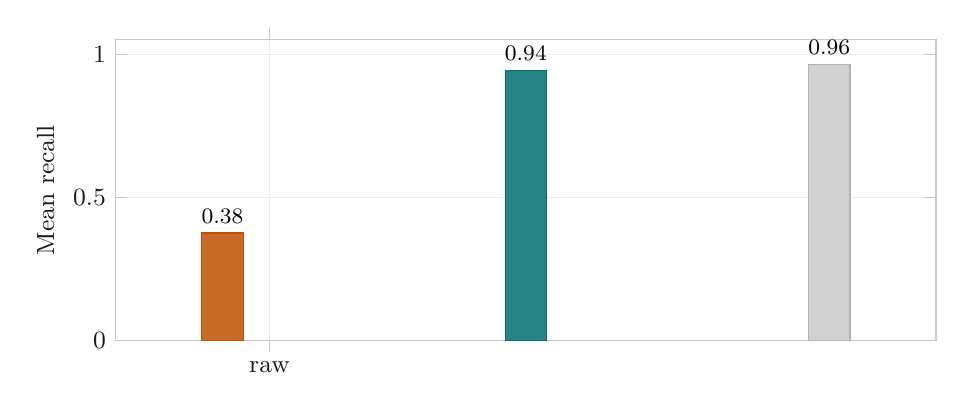
\begin{tikzpicture}
\begin{axis}[ybar,width=12cm,height=5.4cm,bar width=15pt,ymin=0,ymax=1.05,
  ylabel={Mean recall}, symbolic x coords={raw,scaffold,copy ceiling},
  xtick=data, enlarge x limits=0.3, nodes near coords,
  nodes near coords style={font=\footnotesize}]
\addplot[rawstyle] coordinates {(raw,0.375)};
\addplot[scafstyle] coordinates {(scaffold,0.942)};
\addplot[copystyle] coordinates {(copy ceiling,0.964)};
\end{axis}\end{tikzpicture}
\caption{Gemini~3.7~Flash, $n=510$. The scaffold arm (0.942) lands just under the \emph{copy ceiling}
(0.964)---the recall a no-op extractor of the injected context would already achieve. The $+0.57$
raw$\to$scaffold uplift is almost entirely answer exposure, not reasoning over structure.}
\label{fig:anchor}
\end{figure}

\subsection{Ten models: gain over copy}\label{sec:tenmodel}
Table~\ref{tab:sweep} runs the identical paired design across ten models from five providers under one
deterministic configuration. Every model shows a large raw$\to$scaffold uplift ($+0.57$ to $+0.78$)
and every model lands just under the copy ceiling: scaffold recall spans 0.897--0.942 against a
ceiling of \textbf{0.964} that is a property of the questions and the injected context---not the
model---and is therefore identical across the row. The raw uplift is a near-constant restatement of
exposed gold; it does not separate the models.

The signed \textbf{gain over copy} does. It is negative for all ten (Figure~\ref{fig:gain}), from
$-0.067$ (Gemini~2.5~Flash-Lite) to $-0.022$ (Gemini~3.7~Flash): on this lexical metric no model
recovers gold \emph{beyond} what the exposure check already finds, so they differ only in how much
surfaced gold they \emph{drop}. The ordering is interpretable and tracks recency and capability
rather than provider---the newest, strongest models (Gemini~3.7 and 3.5~Flash, Claude~Haiku~4.5) sit
closest to the ceiling (most faithful restatement), while older or smaller models
(Gemini~2.5~Flash-Lite, GPT-4.1-mini, Mistral-Small-24B) lose measurably more. The rank order of gain
tracks that of raw capability, not scaffold recall (which is flat, $0.897$--$0.942$): the instrument
is reading a model property the headline uplift hides. Two models carried transport-level truncations
under the fixed 2048-token budget (GLM-4.6: 174 truncated, 5 retried; Gemini~2.5~Flash-Lite: 16
truncated), recorded per row rather than hidden.

\begin{table}[t]\centering\small
\caption{Ten models, one deterministic configuration, $n=510$ (seed 42), sorted by gain over copy
(scaffold recall $-$ copy ceiling). The copy ceiling (0.964) is a property of the questions and the
injected context and is identical across models. The interval shown is the domain-clustered block
bootstrap (the wider, primary one).}
\label{tab:sweep}
\begin{tabular}{lccccc}
\toprule
Model & Raw & Scaffold & Uplift [clustered 95\% CI] & Ceiling & Gain \\
\midrule
Gemini 3.7 Flash      & 0.375 & 0.942 & $+0.567$ $[+0.524,+0.611]$ & 0.964 & \gainneg{-0.022} \\
Gemini 3.5 Flash-Lite & 0.323 & 0.938 & $+0.615$ $[+0.565,+0.667]$ & 0.964 & \gainneg{-0.026} \\
Claude Haiku 4.5      & 0.151 & 0.934 & $+0.783$ $[+0.741,+0.827]$ & 0.964 & \gainneg{-0.031} \\
GLM-4.6               & 0.243 & 0.928 & $+0.685$ $[+0.641,+0.727]$ & 0.964 & \gainneg{-0.036} \\
DeepSeek-Chat         & 0.347 & 0.924 & $+0.578$ $[+0.532,+0.622]$ & 0.964 & \gainneg{-0.040} \\
Llama-3.3-70B         & 0.227 & 0.916 & $+0.688$ $[+0.632,+0.738]$ & 0.964 & \gainneg{-0.049} \\
Qwen-2.5-72B          & 0.309 & 0.914 & $+0.605$ $[+0.562,+0.649]$ & 0.964 & \gainneg{-0.050} \\
Mistral-Small-24B     & 0.285 & 0.906 & $+0.621$ $[+0.558,+0.682]$ & 0.964 & \gainneg{-0.058} \\
GPT-4.1-mini          & 0.162 & 0.905 & $+0.743$ $[+0.697,+0.787]$ & 0.964 & \gainneg{-0.060} \\
Gemini 2.5 Flash-Lite & 0.227 & 0.897 & $+0.670$ $[+0.623,+0.716]$ & 0.964 & \gainneg{-0.067} \\
\bottomrule
\end{tabular}
\end{table}

\begin{figure}[t]\centering
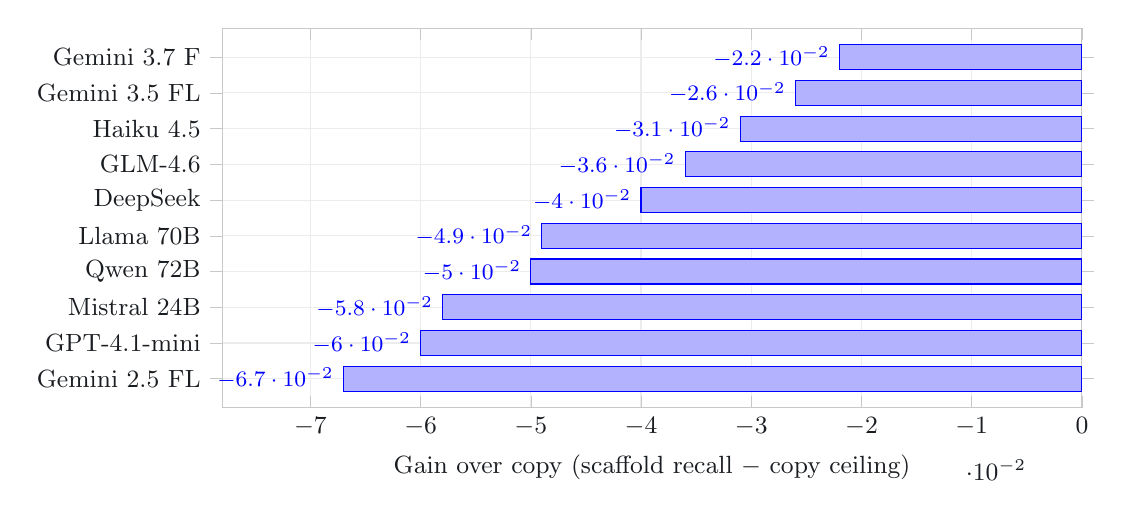
\begin{tikzpicture}
\begin{axis}[xbar,width=12.5cm,height=6.4cm,bar width=9pt,xmin=-0.078,xmax=0,
  xlabel={Gain over copy (scaffold recall $-$ copy ceiling)}, enlarge y limits=0.09,
  symbolic y coords={Gemini 2.5 FL,GPT-4.1-mini,Mistral 24B,Qwen 72B,Llama 70B,DeepSeek,GLM-4.6,Haiku 4.5,Gemini 3.5 FL,Gemini 3.7 F},
  ytick=data, nodes near coords, nodes near coords style={font=\footnotesize},
  every node near coord/.append style={anchor=east},
  every axis plot/.append style={fill=burnt!80,draw=burnt}]
\addplot coordinates {(-0.067,Gemini 2.5 FL) (-0.060,GPT-4.1-mini) (-0.058,Mistral 24B) (-0.050,Qwen 72B) (-0.049,Llama 70B) (-0.040,DeepSeek) (-0.036,GLM-4.6) (-0.031,Haiku 4.5) (-0.026,Gemini 3.5 FL) (-0.022,Gemini 3.7 F)};
\end{axis}\end{tikzpicture}
\caption{Signed gain over copy for all ten models---negative throughout. No model exceeds the copy
ceiling on the lexical metric; the spread ($-0.067$ to $-0.022$) is the axis that separates them
where the near-identical raw uplift does not. Models nearest zero (top) restate the vetted facts
most faithfully.}
\label{fig:gain}
\end{figure}

\subsection{The production-node paired study}\label{sec:live}
The ten-model sweep varies the model with a fixed offline scaffold; the deployment question is whether
the \emph{shipped} node---live retrieval, confidence gate, injection authority and all---moves answer
quality when the model is held constant. Study~2 answers it: Qwen3.8-27B on the reference host,
identical decoding, the only difference being whether the request passes through the Loom node
(\emph{loom}) or hits the backend directly (\emph{raw}), scored $0$--$5$ by the cross-family GPT judge
of \S\ref{sec:method}. Table~\ref{tab:live} reports the paired result per set and pooled.

Pooled over $n=114$, the loom path lifts judged quality by $\mathbf{+0.27}$ points
($[+0.11,+0.45]$, Wilcoxon $p=0.0036$, Cliff's $\delta=0.14$), winning 24 pairs, losing 8 and tying
82. The effect concentrates where the corpus is deep: on the \emph{arcane} set the lift is
$\mathbf{+0.79}$ ($[+0.17,+1.42]$, $p=0.033$, Holm-adjusted $p=0.099$, $\delta=0.29$); on the
sparsely-covered \emph{thin} set it is a positive but non-significant $+0.30$ ($[-0.03,+0.63]$); and
on the out-of-domain \emph{general} set it is a negligible $+0.05$ whose interval $[0.00,+0.13]$ sits
entirely inside the pre-registered $\pm0.25$ equivalence margin---non-regression established by
CI-inclusion, not merely by a non-significant difference (the TOST reading; \S\ref{sec:ood}). The
gradient---large where curation is deep, vanishing where the corpus is thin or the question is
off-domain---is exactly the signature a genuine grounding effect should show, and the opposite of what
a uniform prompt-formatting artefact would produce.

The telemetry corroborates that the gate behaves as designed. Injection engagement is $95.8\%$ on
arcane, $100\%$ on thin, and drops to $78.3\%$ on general---the gate declining to inject on roughly a
fifth of off-domain questions, the mechanism behind the general-set null. Median injected context is
$\approx1{,}200$--$1{,}300$ tokens across sets. Latency is at parity on the sets that matter for the
claim: arcane medians $89.8$\,s (loom) versus $93.4$\,s (raw), general $66.0$ versus $65.7$\,s; the
thin set alone runs slower under loom ($172.4$ versus $145.2$\,s), consistent with its full engagement
and longer scaffolds, and we report it rather than average it away.

\begin{table}[t]\centering\small
\caption{Study~2, the production-node paired study: Qwen3.8-27B, model held constant, loom versus raw
serving path, judged $0$--$5$ by a cross-family GPT judge. Paired mean difference with seeded
10{,}000-resample bootstrap 95\% CI, two-sided Wilcoxon $p$ (Holm-adjusted across the three sets),
Cliff's $\delta$, and win/loss/tie counts. Complete-case after budget-exhaustion re-runs
(\S\ref{sec:results}).}
\label{tab:live}
\begin{tabular}{lcccccc}
\toprule
Set & $n$ & $\Delta$ (loom$-$raw) & 95\% CI & $p$ (Holm) & $\delta$ & W/L/T \\
\midrule
arcane           & 24  & \gainpos{0.79} & $[+0.17,+1.42]$ & 0.033 (0.099) & 0.29 & 10/3/11 \\
thin             & 30  & \gainpos{0.30} & $[-0.03,+0.63]$ & 0.118 (0.237) & 0.23 & 12/5/13 \\
general          & 60  & \gainpos{0.05} & $[\phantom{+}0.00,+0.13]$ & 0.180 (0.237) & 0.03 & 2/0/58 \\
\midrule
\textbf{pooled}  & 114 & \gainpos{0.27} & $[+0.11,+0.45]$ & \textbf{0.0036} & 0.14 & 24/8/82 \\
\bottomrule
\end{tabular}
\end{table}

\subsection{Negative controls: attributing the gain}\label{sec:controls}
The live lift and the ten-model delivery both invite one objection: that the gain is lexical overlap
between answer and injected block, not knowledge transfer. The four control arms of
\S\ref{sec:ceiling-controls} test it directly, each holding the model and question fixed and
perturbing only the injected scaffold, fetched verbatim from the LLM-free \texttt{/loom/scaffold}
endpoint. Table~\ref{tab:controls} reports the pooled (arcane\,$+$\,thin) contrasts; we read them as
lower-confidence, complete-case comparisons for the attrition reasons of \S\ref{sec:results}.

Three results triangulate the attribution. First, a \textbf{sanity check}: serving the exact block
through the bare model (\emph{true}) reproduces the live \emph{loom} arm---loom\,$-$\,true is
$-0.06$ $[-0.38,+0.25]$, indistinguishable from zero, confirming the serving path adds nothing beyond
the block it injects. Second, the \textbf{content effect is real}: true\,$-$\,raw is $+0.59$
$[+0.16,+1.06]$ ($p=0.026$)---injecting the served block lifts judged quality well above the bare
model. Third, and decisively, the \textbf{placebo collapses}: an equally well-formed, on-corpus
scaffold drawn from a \emph{different} question (\emph{irrelevant}) moves nothing---irrelevant\,$-$\,raw
is $+0.04$ $[-0.54,+0.57]$ ($p=0.73$). Subtracting the placebo from the content arm isolates the
content-specific component, true\,$-$\,irrelevant\,$=+0.35$ $[0.00,+0.78]$ ($p=0.091$): the majority
of the raw-to-served lift is bound to \emph{which} block is injected, not to the mere presence of
ontology-shaped text.

\paragraph{The placebo had to be verified inert.} This conclusion depends entirely on the irrelevant
arm being a true placebo, and our first attempt was not. Constructing the ``different question'' donor
by a shift-by-one derangement over the engaged items left donors in the \emph{same} domain cluster as
their targets---so the ``irrelevant'' scaffold routinely shared vocabulary and neighbouring concepts
with the gold, and behaved like a weak content arm rather than a placebo. We rebuilt the derangement
under a seed-IRI-disjointness constraint (every donor scaffold verified to share no seed IRI, and thus
no seed class, with its target's gold) and only then did the arm collapse to $\approx0$. A placebo that
is assumed inert rather than verified inert silently inflates the very baseline it is meant to
control; the fix was cheap and the lesson is general.

Masking and shuffling lose comparatively little. Replacing every seed-class \emph{name} with
\texttt{Entity-$k$} (\emph{masked}) still beats raw by $+0.42$ (ns, wide CI), and shuffling the block's
sentences (\emph{shuffled}) by $+0.25$ (ns): the graded facts, not the surface names or their order,
carry most of the signal---consistent with a judge grading factual content over lexical form. Finally,
the effect is a \textbf{curation-depth gradient}: per set, true\,$-$\,raw is $+0.95$ $[+0.37,+1.63]$
($p=0.018$) on the deep arcane set but only $+0.08$ $[-0.46,+0.62]$ (ns) on the thin set. Where the
corpus is rich the served block transfers real knowledge; where it is sparse there is little to
transfer---the same gradient the live study shows, recovered independently through the controls.

\begin{table}[t]\centering\small
\caption{Negative-control contrasts, pooled arcane\,$+$\,thin, judged $0$--$5$, paired mean difference
with seeded bootstrap 95\% CI and two-sided Wilcoxon $p$. Complete-case over surviving pairs; the
control arms were not retried at the larger budget, so $n$ varies by arm (\S\ref{sec:results}). Read
top to bottom: the serving path adds nothing (loom$-$true~$\approx0$); the served block lifts quality
(true$-$raw); the same-shaped placebo does not (irrelevant$-$raw~$\approx0$); the content-specific
residual is true$-$irrelevant.}
\label{tab:controls}
\begin{tabular}{lcccc}
\toprule
Contrast & $n$ & $\Delta$ & 95\% CI & Wilcoxon $p$ \\
\midrule
loom $-$ true             & 32 & $-0.06$ & $[-0.38,+0.25]$ & 0.81 \\
true $-$ raw              & 32 & \gainpos{0.59} & $[+0.16,+1.06]$ & 0.026 \\
masked $-$ raw            & 33 & \gainpos{0.42} & $[-0.09,+0.94]$ & 0.15 \\
shuffled $-$ raw          & 36 & \gainpos{0.25} & $[-0.39,+0.89]$ & 0.42 \\
irrelevant $-$ raw        & 28 & \gainpos{0.04} & $[-0.54,+0.57]$ & 0.73 \\
true $-$ irrelevant       & 23 & \gainpos{0.35} & $[\phantom{+}0.00,+0.78]$ & 0.091 \\
\midrule
\multicolumn{5}{@{}l@{}}{\emph{Per set (true $-$ raw):} arcane $+0.95$ $[+0.37,+1.63]$, $p=0.018$; thin $+0.08$ $[-0.46,+0.62]$, ns.}\\
\bottomrule
\end{tabular}
\end{table}

\subsection{Out-of-domain: the gate holds}\label{sec:ood}
Two instruments agree that grounding does not cost anything on the general questions a model already
answers. The v1 judged arm graded a 60-question out-of-domain set $0$--$5$ against frontier gold with a
cross-family judge across five models: every paired harness$-$bare delta's 95\% interval includes
zero---all questions $-0.05$ $[-0.11,0.00]$; off-domain $-0.09$ $[-0.25,+0.02]$; and even the
pre-specified worst case, off-domain questions on which the gate mis-fired and injected anyway,
$-0.23$ $[-0.63,+0.05]$, still spanning zero (Table~\ref{tab:ood}). The mechanism is the gate: when it
correctly judged a query off-domain and skipped (60 of 100 off-domain gradings) the harnessed answer
was identical to bare; the only degradation appeared when it over-fired, and it concentrated on the
weakest model. The production study adds the equivalence reading the v1 arm lacked: the general-set
$\Delta=+0.05$ $[0.00,+0.13]$ lies wholly inside the pre-registered $\pm0.25$ TOST margin, so
non-regression is established by CI-inclusion rather than inferred from a non-significant difference.
As in v1 we report ``no jaggedness detected'' rather than ``zero effect''---the intervals are wide and
bound the regression near zero, they do not prove its absence.

\begin{table}[t]\centering\small
\caption{Out-of-domain non-regression (v1 judged arm): paired harness$-$bare quality delta (judge
$0$--$5$ vs frontier gold), five models, seeded paired bootstrap 95\% CI. Every interval includes
zero. The worst case is off-domain questions where the confidence gate mis-fired and injected anyway;
the last row is where it correctly skipped.}
\label{tab:ood}
\begin{tabular}{lccc}
\toprule
Subset & Mean $\Delta$ & 95\% CI & $n$ pairs \\
\midrule
All general questions              & $-0.05$ & $[-0.11,\ 0.00]$ & 300 \\
\quad adjacent                     & $+0.01$ & $[-0.02,\ 0.05]$ & 100 \\
\quad in-domain-general            & $-0.06$ & $[-0.14,\ 0.00]$ & 100 \\
\quad off-domain                   & $-0.09$ & $[-0.25,\ 0.02]$ & 100 \\
Off-domain, gate mis-fired (worst) & $-0.23$ & $[-0.63,\ 0.05]$ & 40 \\
Off-domain, gate skipped (correct) & $+0.00$ & ---              & 60 \\
\bottomrule
\end{tabular}
\end{table}

\section{Analysis: Exposure, not Reasoning}\label{sec:analysis}
The results across both studies say one thing in several registers: the uplift a graph-grounding layer
delivers over a private corpus is overwhelmingly \emph{exposure}---faithful delivery of curated facts
the model was shown---and not \emph{reasoning} over injected structure. This section reads that claim
off the instrument, then draws the two engineering consequences that reframe how such a system should
be built and evaluated.

\paragraph{The headline is delivery fidelity, and the instrument is what reveals it.} The ten-model
sweep is the cleanest statement: raw uplift is huge and near-constant ($+0.57$ to $+0.78$), yet gain
over copy is small and \emph{uniformly negative} ($-0.067$ to $-0.022$). Read against a bare-model
baseline every model looks transformed; read against the copy ceiling none exceeds what a verbatim
copy of its own context already exposes, and they separate only by how much surfaced gold they drop.
The number the field would report as the achievement (the uplift) is the number that carries the least
information about the model; the number that discriminates (gain over copy) is invisible without the
ceiling. That inversion is the whole case for reporting the ceiling as standard.

\paragraph{The live decomposition confirms it is content, not form.} The production controls take the
same conclusion from headline to mechanism. The served block lifts judged quality (true\,$-$\,raw
$+0.59$); a same-shaped, on-corpus but wrong block does not (irrelevant\,$-$\,raw $+0.04$); the
content-specific residual is $+0.35$; and masking names ($+0.42$) or shuffling sentences ($+0.25$)
costs comparatively little. The facts carry the effect; the entity names and their order do not. Three
caveats keep this honest: the arms are complete-case over unequal survivor sets, the contrasts do not
sum arithmetically (different survivors per arm), and several are non-significant with wide intervals.
But the qualitative pattern---content-specific lift present, verified-inert placebo absent---is exactly
what ``exposure, faithfully delivered'' predicts and what ``any ontology-shaped text primes the model''
does not. The placebo episode is the load-bearing methodological point: the effect only appeared clean
once the irrelevant donor was \emph{verified} seed-IRI-disjoint; a placebo assumed inert had leaked
domain vocabulary and manufactured a spurious baseline.

\paragraph{Consequence 1: the copy ceiling is a regime detector---compute it before you architect.}
The ceiling is not only a post-hoc control; it is a design-time diagnostic. Compute it on a
representative question set \emph{before} choosing an architecture. A near-1 ceiling (our setting:
0.964) means the corpus already contains the answer verbatim---this is a \emph{serving regime}, where
verbatim retrieval wins and generative re-encoding can only lose fidelity, so the engineering target is
faithful delivery and the metric is gain over copy. A low ceiling means the answer is \emph{not}
present as-is and must be composed across retrieved pieces---a \emph{synthesis regime}, where
GraphRAG-style machinery (community summaries, multi-hop traversal, GNN soft-prompts) can earn its
keep. The essential discipline is that in a synthesis regime that machinery must be measured
\emph{above the ceiling}, not above a bare-model baseline: an uplift over the bare model in a
high-ceiling setting is delivery masquerading as reasoning. Much reported graph-RAG gain is, we
suspect, un-diagnosed serving-regime exposure; the ceiling is the cheap test that tells the two apart
before a team builds the expensive apparatus.

\paragraph{Consequence 2: value concentrates at curation, and the instrument doubles as a promotion
gate.} If the model contributes delivery and the corpus contributes the answer, then the leverage is
upstream, at curation time---which is where the economics of a private corpus already put it, since the
curation is amortised once and re-paid on no query. This gives the instrument a second use. An
automated extraction candidate (for example a block proposed by OntoCast~\cite{ontocast}, analysed here
purely as a third-party upstream producer) can be scored by the copy ceiling of the questions its block
is meant to answer: a candidate whose block drives the ceiling toward 1 is answer-complete and worth
promoting; one that does not is not yet ready. The same quantity that audits the serving layer thus
grades the ingestion layer---answer-completeness of a block $\approx$ its copy ceiling---turning the
control into a governance gate at the boundary where value is actually created.

\paragraph{The honest discovery arc.} We did not set out to write this. We built the serving node
first, saw large uplift, and worried we had merely reinvented GraphRAG with a nicer provenance story.
The copy ceiling began as an adversarial question we put to our own result---\emph{is any of this
reasoning, or is it all exposure?}---and the honest answer, uniformly negative gain over copy across
ten models and a placebo that collapses once verified inert, is that it is exposure. For a
private-knowledge product that is not a disappointment but the specification met: trustworthy because
the source is vetted, attributable because the generation is named, and cheap because the curation is
paid once. The contribution is the instrument that let us tell the difference, and the discipline of
reporting it.

\section{The Multivariate Bar}\label{sec:bar}
No single number is the deployable target. The bar introduced in \S\ref{sec:setting} is conjunctive
across four axes; Table~\ref{tab:bar} states each, the instrument that measures it, and this work's
honest status against it. We shrink rather than inflate the scorecard: two axes are measured here, two
are specified and not yet closed.

\begin{table}[t]\centering\small
\caption{The multivariate bar and this work's status. A deployable private-knowledge system must clear
all four \emph{together}; the axes are measured on different instruments, so no single number
establishes the conjunction.}
\label{tab:bar}
\renewcommand{\arraystretch}{1.2}
\begin{tabularx}{\textwidth}{@{}>{\raggedright\arraybackslash}p{3.5cm} >{\raggedright\arraybackslash}X >{\raggedright\arraybackslash}p{3.6cm}@{}}
\toprule
Axis & Instrument \& evidence & Status \\
\midrule
1. In-domain delivery fidelity & Copy ceiling / gain over copy: ten models $-0.067$ to $-0.022$; live loom$-$raw $+0.27$ pooled, $+0.79$ arcane & \textbf{Measured} (v1 $+$ live) \\
2. Out-of-domain non-regression & Judged $\Delta$ vs frontier gold: v1 all CIs include zero (worst $-0.23$ $[-0.63,+0.05]$); live general $+0.05$ $[0.00,+0.13]$ inside $\pm0.25$ TOST margin & \textbf{Measured} (v1 $+$ live) \\
3. Beats web search in-domain & Same model grounded in live web results vs curated scaffold, identical question set & Specified; not measured \\
4. Attribution precision & Per-answer generation $+$ confidence already emitted; precision metric to close ``faithful'' $\to$ ``attributable'' & Specified; not measured \\
\bottomrule
\end{tabularx}
\end{table}

Axes~1 and~2 are the conjunction this paper establishes: excellent, attributable delivery where the
corpus is authoritative, \emph{and} no detected regression where it is not, measured on two different
instruments so the pairing is not an artefact of one metric. Axis~3 (the right baseline is a
web-grounded arm on the same questions, not the bare model) and axis~4 (a reported attribution-precision
figure) are designed and unmeasured; we name them as open rather than imply the bar is cleared. The
value of stating the full bar is that it prevents the in-domain number from being read as the whole
claim---the failure mode the copy ceiling exists to prevent.

\section{Limitations and Threats to Validity}\label{sec:limits}
\begin{itemize}[topsep=2pt,itemsep=2pt,leftmargin=1.4em]
\item \textbf{Single corpus.} Both studies run on one curated ontology in one broad domain. The copy
ceiling and its decomposition are corpus-general in construction, but the magnitudes---a 0.964 ceiling,
a $+0.27$ live lift---are properties of this corpus and do not transfer as numbers.
\item \textbf{Single-family judge.} Study~2's judge is a single GPT-family model. It is cross-family
from the Qwen candidate (avoiding self-preference) but is not a panel; a judge idiosyncrasy would
propagate. The gold references mitigate but do not eliminate this.
\item \textbf{Complete-case control attrition.} The control arms were not retried at the larger budget
and carry $36$--$50\%$ empty attrition at 1536, so every control contrast is complete-case over unequal
survivor sets. The arms do not sum arithmetically, several are non-significant with wide intervals
(shuffled$-$raw, masked$-$raw, true$-$irrelevant), and the attribution rests on the \emph{pattern}
across arms rather than any single contrast.
\item \textbf{Small per-set $n$ for controls.} Per-set control contrasts run on $n=8$--$21$; the
curation-depth gradient (arcane true$-$raw $+0.95$ significant, thin $+0.08$ ns) is suggestive, not
definitively estimated, and the thin-set nulls are as consistent with low power as with no effect.
\item \textbf{Lexical scorer for the v1 axes.} The ten-model gain-over-copy and in-domain recall use a
lexical title matcher that under-counts paraphrase; absolute recall is a lower bound and gain over copy
is framed as a lower-bound estimand. Only Study~2 uses the semantic judge.
\item \textbf{Semantic fallback disabled throughout.} The HNSW semantic retrieval path was off in every
reported run---its document-embedding recall (0.816) is below the 0.87 design floor (a red gate we
report rather than relax)---so the loom arm is lexical-retrieval only. A query-shaped embedding that
clears the floor could change the engagement and thin-set numbers.
\item \textbf{Single production model.} Study~2 holds the model at Qwen3.8-27B. The serving-path effect
is isolated cleanly, but its magnitude under other backends is unmeasured; the ten-model sweep varies
the model only for the offline scaffold, not the live node.
\item \textbf{Three excluded questions.} Three questions empty at 4096 in both arms are dropped
(complete-case $n=114$). The exclusion is symmetric across arms but is a departure from intention-to-treat.
\item \textbf{Two axes of the bar unmeasured.} The web-search baseline (axis~3) and attribution
precision (axis~4) are specified and not measured here; the deployable claim is not yet fully closed.
\end{itemize}

\section{Conclusion}\label{sec:conclusion}
Grounding evaluations whose gold is derived from the injected corpus should \textbf{report a copy
ceiling as standard.} It is a cheap, per-item, model-free quantity---the recall a verbatim copy of the
shown context already achieves---and the signed gain over copy it defines separates faithful delivery
of exposed facts from reasoning over injected structure, a distinction a bare-model baseline cannot
make. Across ten models the gain is uniformly negative; a production paired study lifts judged quality
by $+0.27$ pooled and $+0.79$ where curation is deep; and a negative-control decomposition binds that
lift to scaffold \emph{content}, with the placebo collapsing once verified seed-disjoint. The reusable
method is the pair: \emph{the ceiling plus a verified-inert placebo}, computed before architecting to
tell a serving regime (verbatim retrieval wins) from a synthesis regime (where heavier machinery must
be measured above the ceiling, not above the bare model). And the economics follow the measurement:
value concentrates upstream at curation, where the same instrument doubles as a promotion gate for
extraction candidates. For a private corpus the goal was never a model that reasons its way to answers
it never saw---it is a model that delivers vetted knowledge faithfully, attributably and cheaply, and
an instrument honest enough to prove that is what it does.

\printbibliography

\end{document}
